\documentclass{article}
\usepackage{CJKutf8}
\usepackage{tikz,pgffor}
\usetikzlibrary{shadows}
\usetikzlibrary{arrows}
\usetikzlibrary{calc,intersections,through,backgrounds}
\usepackage{ifthen}
\begin{document}
\begin{CJK}{UTF8}{gbsn}%{gkai} %


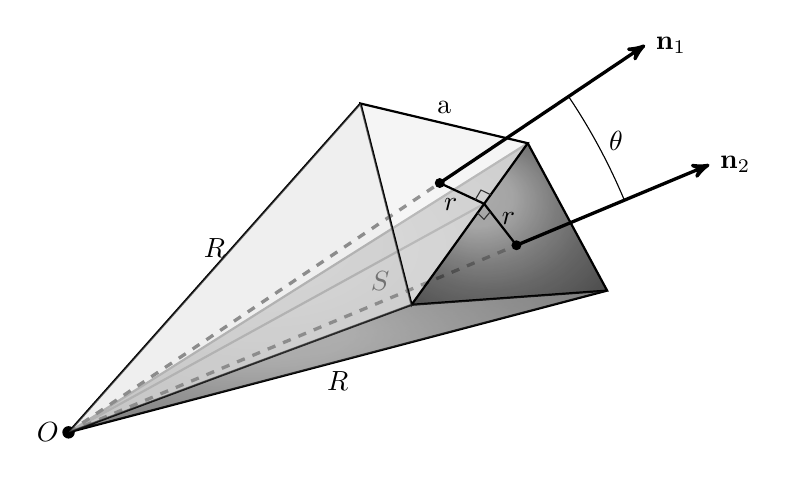
\begin{tikzpicture}[scale = 0.9,
    axis/.style={very thick, ->, >=stealth'},
    important line/.style={thick},
    dashed line/.style={dashed, thin},
    pile/.style={thick, ->, >=stealth', shorten <=2pt, shorten
    >=2pt},
    every node/.style={color=black}]
    \coordinate (O) at (0,0);
    \coordinate (A) at (4.12,4.64);
    \coordinate (B) at (4.84,1.8);
    \coordinate (C) at (6.48,4.08);
    \coordinate (D) at (7.6,2.0);
    \coordinate (e) at (33.89:6.31);
    \coordinate (f) at (22.67:6.85);
    \coordinate (X) at ($ (B)!.625!(C) $);

    \filldraw[fill=gray!20,draw=gray!20,opacity=0.2] (O) -- (A) -- (C) -- cycle;
    \filldraw[ball color= gray!20,draw=gray!80,opacity=0.2] (O) -- (D) -- (C) -- cycle;
    \filldraw[fill=gray,draw=gray,opacity=0.2] (O) -- (B) -- (C) -- cycle;
    \draw [thick, gray] (O) -- (C) (O)-- node[near end,below]{$S$}(X); 
    
    \draw [very thick, dashed, black!80] (O) -- (e) (O) -- (f);
    \filldraw[fill=gray!10,draw=gray!10,opacity=0.5] (A) -- (C) -- (B) -- cycle;
    \filldraw[ball color= gray!20,draw=gray!80,opacity=0.5] (D) -- (C) -- (B) -- cycle;
    

    \draw[thick] (A) -- node[above] {a} (C) -- (B) -- cycle;
    
    \draw[thick] (C)-- (D) -- (B); 
    \draw[thick] (O) -- node[above]{$R$} (A) 
          (O) -- (B) 
          (O) -- node[below]{$R$} (D);
\draw[thick] (e) -- node[near start,below] {$r$} (X) (f) --  node[near start, above] {$r$} (X);
    \draw[black!80] ($ (X)!.15!(C) $) -- ($ (X)!.15!(C)!0.08!-80:(B) $) -- ($ (X)!.2!(e) $)
($ (X)!-.15!(C) $) -- ($ (X)!-.15!(C)!0.08!80:(B) $) -- ($ (X)!.19!(f) $);
    \draw [axis] (e) -- (33.89:9.8) node[right] {$\mathbf{n}_1$};
    \draw [axis] (f) -- (22.67:9.8) node[right] {$\mathbf{n}_2$};
    \draw (22.67:8.5)  arc(22.67:33.89:8.5) (28:8.75) node{$\theta$};
    \fill (0,0)    node[left]{$O$}    circle (2.5pt) 
          (33.89:6.31) circle (2pt) 
          (22.67:6.85) circle (2pt);
    \filldraw[fill=gray!20,draw=black,opacity=0.5] (O) -- (A) -- (B) -- cycle;
    \filldraw[ball color= gray!20,draw=black,opacity=0.2] (O) -- (D) -- (B) -- cycle;

\end{tikzpicture}
%\end{figure}
\end{CJK}
\end{document} 
